%%
%% UTF-8       UTF-8      UTF-8       UTF-8       UTF-8       UTF-8
%% UTF-8       UTF-8      UTF-8       UTF-8       UTF-8       UTF-8
%%
%% XeLaTeX  XeLaTeX  XeLaTeX  XeLaTeX  XeLaTeX  XeLaTeX  XeLaTeX  XeLaTeX  
\lccode`\-=`\-
%\defaulthyphenchar=127
% \documentclass[11pt,a4paper,oneside]{extarticle}
\documentclass[12pt,a4paper,twoside]{article}


% ---------------------------------------------------------
% Cores básicas e fundo de página
% ---------------------------------------------------------
\usepackage[xetex,dvipsnames,svgnames,table]{xcolor}

% Cores definidas por CMYK
% \definecolor{fondpaille}{cmyk}{0,0.02,0.2,0}
\definecolor{fondpaille}{cmyk}{0, 0.0118, 0.1176, 0, 0.01} %cmyk(0%, 2.75%, 23.53%, 0%, 1%)
\definecolor{ferrugem}{cmyk}{0, 0.4457, 0.75, 0.6392}

% Cores definidas por hexadecimal
\definecolor{moleskin}{HTML}{FFF8DC}
\definecolor{laranja}{HTML}{F07241}
\definecolor{marron}{HTML}{800000}
\definecolor{lovely}{HTML}{C04848}
\definecolor{click}{HTML}{480048}
\definecolor{tinta-velha}{HTML}{4e4643}
\definecolor{Browned_Cherry}{HTML}{910831}
\definecolor{azul}{HTML}{000080}

% Cores da capa
\definecolor{BLACK}{HTML}{000000}
\definecolor{ELECTRICRED}{HTML}{DD0000}
\definecolor{TANGERINYELLOW}{HTML}{FFCE00}

% Cor consolidada para texto principal
\colorlet{cor-da-tinta}{ferrugem}
\newif\ifferrugem
\ferrugemfalse

% Cor de fundo da página
\pagecolor{fondpaille}

% ---------------------------------------------------------
% Fontes
% ---------------------------------------------------------
\usepackage{fontspec} % XeLaTeX/LuaLaTeX fonts
\setmainfont{EBGaramond}[ % Tudo junto, não 'EB Garamond'
  %% TECTONIC:  %%  %%  %%  %%  %%
  Path=./auxiliares/ebgaramond/,
  Extension=.ttf,
  UprightFont=*-Regular,
  BoldFont=*-Bold,
  ItalicFont=*-Italic,
  BoldItalicFont=*-BoldItalic,
  %%  %%  %%  %%  %%  %%  %%  %%  %%
  Numbers=OldStyle,
  RawFeature={
    -aalt,
    -c2pc,
    -c2sc,
    -case,
    +dlig,
    -frac,
    -hist,
    +hlig,
    +kern,
    +liga,
    +mark,
    +mkmk,
    +onum,
    +pnum,
    +ss05,
    +cv06
  }
]
\usepackage[math-style=ISO, bold-style=ISO]{unicode-math}
% \setmathfont{OldStandard-Math.otf}
% \setmathfont{Garamond-Math.otf}[StylisticSet={5,6,7,9}]
\setmathfont{NewCMMath-Book.otf}

% ---------------------------------------------------------
% Línguas e hifenização
% ---------------------------------------------------------
\usepackage{polyglossia}
\setdefaultlanguage{portuguese}
\PolyglossiaSetup{portuguese}{indentfirst=true}
\setotherlanguages{english,french} % TECTONIC: 'german' não funciona

% ---------------------------------------------------------
% Tipografia avançada
% ---------------------------------------------------------
\usepackage{microtype}      % ajustes de tipografia
\usepackage[bottom]{footmisc} % pés de página alinhados ao fundo
\linespread{1.3}            % espaçamento de linha

% ---------------------------------------------------------
% Matemática e símbolos
% ---------------------------------------------------------
\usepackage{amsmath,dsfont,mathrsfs,wasysym}
\usepackage[makeroom,thicklines]{cancel} % para riscar
\usepackage{esvect}       % vetores

% ---------------------------------------------------------
% Código-fonte e Python
% ---------------------------------------------------------
\usepackage{fvextra}
\usepackage{fancyvrb}
\usepackage{listings}
% \usepackage{pythontex}  TECTONIC: Não é compatível

% ---------------------------------------------------------
% Gráficos e figuras
% ---------------------------------------------------------
\usepackage{graphicx}
\usepackage{svg}
\usepackage{tikz}
\usepackage{tkz-fct}
\usepackage{tikzpagenodes}
\usepackage{circuitikz}
\usepackage{pgfplots,pgfplotstable}
\pgfplotsset{compat=newest}
\usetikzlibrary{
  calc,
  positioning,
  automata,
  arrows,
  shadows,
  shapes.multipart,
  matrix,
  backgrounds,
  decorations.pathreplacing,
  fit,
  plotmarks,
  tikzmark
}
\pgfdeclarelayer{background}
\pgfdeclarelayer{foreground}
\pgfsetlayers{background,main,foreground}

% ---------------------------------------------------------
% Tabelas avançadas
% ---------------------------------------------------------
\usepackage{array,longtable,booktabs,bigstrut,tabularx,seqsplit}

% ---------------------------------------------------------
% Notas de rodapé e citações
% ---------------------------------------------------------
\usepackage{csquotes}
\usepackage[toc,page]{appendix}
\renewcommand\appendixpagename{Apêndices}
\usepackage[
  backend=biber,
  style=numeric-comp,
  language=auto,
  natbib=false,
  block=space,
  isbn=false,
  url=true,
  doi=false,
  mcite=true,
  eprint=false,
  sorting=none
]{biblatex}
\addbibresource{bibliografia.bib}

% Formato das notas de rodapé
\renewcommand{\thefootnote}{\alph{footnote}}
\makeatletter
\renewcommand\@makefnmark{\@textsuperscript{\normalfont(\@thefnmark)}}
\makeatother
\long\def\symbolfootnote[#1]#2{%
  \begingroup
  \def\thefootnote{\fnsymbol{footnote}}
  \footnote[#1]{#2}
  \endgroup
}

% ---------------------------------------------------------
% Secções e sumário
% ---------------------------------------------------------
\usepackage{titlesec}
\usepackage{tocloft}
\usepackage{etoolbox}

% Novos níveis de secção
\titleclass{\subsubsubsection}{straight}[\subsubsection]
\titleclass{\subsubsubsubsection}{straight}[\subsubsubsection]
\newcounter{subsubsubsection}[subsubsection]
\newcounter{subsubsubsubsection}[subsubsubsection]
\renewcommand{\thesubsubsubsection}{\thesubsubsection.\arabic{subsubsubsection}}
\renewcommand{\thesubsubsubsubsection}{\thesubsubsubsection.\arabic{subsubsubsubsection}}

% Formato visual
\titleformat{\subsubsubsection}{\normalfont\normalsize\bfseries}{\thesubsubsubsection}{1em}{}
\titlespacing*{\subsubsubsection}{0pt}{3.25ex plus 1ex minus .2ex}{1.5ex plus .2ex}
\titleformat{\subsubsubsubsection}{\normalfont\normalsize\bfseries}{\thesubsubsubsubsection}{1em}{}
\titlespacing*{\subsubsubsubsection}{0pt}{3.25ex plus 1ex minus .2ex}{1.5ex plus .2ex}

% Sumário detalhado
\renewcommand{\cftsecfont}{\bfseries}
\renewcommand{\cftsubsecfont}{\normalfont}
\renewcommand{\cftsubsubsecfont}{\normalfont}
\makeatletter
\renewcommand{\l@section}{\@dottedtocline{1}{1.5em}{1.5em}}
\renewcommand{\l@subsection}{\@dottedtocline{2}{2.5em}{2em}}
\renewcommand{\l@subsubsection}{\@dottedtocline{3}{4em}{2.5em}}
\newcommand{\l@subsubsubsection}{\@dottedtocline{4}{6em}{3em}}
\newcommand{\l@subsubsubsubsection}{\@dottedtocline{5}{8em}{4em}}
\providecommand*{\toclevel@subsubsubsection}{4}
\providecommand*{\toclevel@subsubsubsubsection}{5}
\makeatother
\setcounter{secnumdepth}{5}
\setcounter{tocdepth}{5}

% ---------------------------------------------------------
% Layout de página
% ---------------------------------------------------------
\usepackage[a4paper,left=2.5cm,right=2.5cm,top=2.5cm,bottom=2.5cm,includehead,includefoot]{geometry}
\usepackage{setspace} % espaçamento de linhas
\usepackage{lettrine,calligra} % letras capitulares
\renewcommand{\LettrineFontHook}{\calligra}
\LettrineTextFont{\itshape}
\setcounter{DefaultLines}{3}

% Prevenção de viúvas e órfãos
\clubpenalty=100
\linepenalty=100
\widowpenalty=100

% Outros ajustes tipográficos
\usepackage{xurl}
\usepackage[hang,small,bf]{caption}
\setlength{\captionmargin}{1.5in}
\renewcommand{\fboxrule}{2pt}

% ---------------------------------------------------------
% Utilitários diversos
% ---------------------------------------------------------
\usepackage{comment}
\usepackage{enumerate}
\newcounter{lastenum}
\newcommand{\storelast}{\setcounter{lastenum}{\value{enumi}}}
\newcommand{\uselast}{\setcounter{enumi}{\value{lastenum}}}
\newcommand\CC{C\nolinebreak[4]\hspace{-.05em}\raisebox{.4ex}{\relsize{-3}{\textbf{++}}}}
\usepackage{rotating}
\usepackage{array}
\usepackage{lastpage}
\usepackage{refcount}
\usepackage{standalone}
\usepackage{relsize}
\usepackage[normalem]{ulem}
\usepackage[most]{tcolorbox}

% ---------------------------------------------------------
% Datas e formatação numérica
% ---------------------------------------------------------
\usepackage[nodayofweek,level]{datetime}
\usepackage[output-decimal-marker={,}]{siunitx}

% ---------------------------------------------------------
% Pacotes de cálculo e exercícios
% ---------------------------------------------------------
\usepackage{xlop}      % cálculo automático

% ---------------------------------------------------------
% Topo e rodapé de páginas (logos e texto)
% ---------------------------------------------------------
\usepackage{eso-pic}

\AddToShipoutPictureBG{%           % Início do bloco que adiciona elementos ao fundo da página
  \ifnum\value{page}>2           % Condição: só aplica a partir da página 3
    \AtPageUpperLeft{%            % Posiciona tudo relativamente ao canto superior esquerdo da página
      \begin{tikzpicture}[remember picture, overlay]% Início do ambiente TikZ sobreposto (overlay) e lembrando posição
        % Linhas superior e inferior
        \draw[line width=0.5pt, color=black] (2.5cm, -3cm) -- (\paperwidth - 2.5cm, -3cm); % Linha horizontal superior
        \draw[line width=0.5pt, color=black] (2.5cm, -\paperheight + 3cm) -- (\paperwidth - 2.5cm, -\paperheight + 3cm); % Linha horizontal inferior
        
        % Conteúdo página ímpar
        \ifodd\value{page}           % Verifica se a página é ímpar
          \node [anchor=west, text depth=0pt] at (2.5cm, -2.7cm){\tiny\href{mailto:luisav.ferreira@gmail.com}{Grupo Disciplinar 510}}; % Texto canto superior esquerdo
          \node [anchor=north east] at (\paperwidth-2.5cm, -2.2cm){
\includegraphics[width=0.05\paperwidth]{logos/aeB05.pdf}}; % Logo canto superior direito
          \node [anchor=west, text height=0pt] at (2.5cm, -\paperheight + 2.7cm){\tiny\href{mailto:luisav.ferreira@gmail.com}{Luís A.V. Ferreira}}; % Texto canto inferior esquerdo
          \node [anchor=west] at (2.5cm, -\paperheight + 2.5cm){\tiny\jobname.tex \smash{\rule[-0.5ex]{0.6pt}{1ex}}}; % Nome do ficheiro e linha decorativa
        % Conteúdo página par
        \else                        % Caso seja página par
          \node [anchor=west, text depth=0pt] at (2.5cm, -2.7cm){
\includegraphics[width=0.05\paperwidth]{logos/aeB05.pdf}}; % Logo canto superior esquerdo
          \node [anchor=east, text depth=0pt] at (\paperwidth - 2.5cm, -2.7cm){\tiny\href{mailto:luisav.ferreira@gmail.com}{Grupo Disciplinar 510}}; % Texto canto superior direito
          \node [anchor=east, text height=0pt] at (\paperwidth - 2.5cm, -\paperheight + 2.7cm){\tiny\href{mailto:luisav.ferreira@gmail.com}{Luís A.V. Ferreira}}; % Texto canto inferior direito
          \node [anchor=east] at (\paperwidth - 2.5cm, -\paperheight + 2.5cm){\tiny\jobname.tex \smash{\rule[-0.5ex]{0.6pt}{1ex}}}; % Nome do ficheiro e linha decorativa
        \fi
      \end{tikzpicture}
    }
  \fi
}

% ---------------------------------------------------------
% hyperref
% ---------------------------------------------------------

\usepackage[%
  bookmarks=true,
  citecolor=black,
  filecolor=black,
  linkcolor=black,
  urlcolor=blue,     % Cor específica para URLs
  unicode=false,
  colorlinks=false,
  plainpages=false,
  pdfpagelabels,
  colorlinks=true,  % Ativa cores em vez de caixas
  xetex]{hyperref} 


\begin{document}
%%%%%%%%%%%%%%%%%%%%%%%%%%%%%%%%%

\begin{titlepage}
	\centering
	
\includegraphics[width=0.15\textwidth]{logos/aeB06.pdf}  \par
	\vspace{1cm}
	{\scshape\LARGE Escola Secundaria José Gomes Ferreira    \par}
	\vspace{1cm}
	{\scshape\Large Física 12º     \par}
	\vspace{1.5cm}
	{\huge\bfseries Modelos de relatório}\par 
	\vspace{2cm}
	{\Large\itshape Nome do aluno}\par
	{\Large\itshape Nº e Turma}\par 
	\vfill
% Bottom of the page
	{\large \today\par}

	
\begin{tikzpicture}[remember picture, overlay]
\draw[line width = 2pt, color=BLACK ] ($(current page.north west) + (.5in,-.5in)$) rectangle ($(current page.south east) + (-.5in,.5in)$);
\draw[line width = 1pt, color=ELECTRICRED ] ($(current page.north west) + (.55in,-.55in)$) rectangle ($(current page.south east) + (-.55in,.55in)$);
\draw[line width = 1pt, color=TANGERINYELLOW ] ($(current page.north west) + (.6in,-.6in)$) rectangle ($(current page.south east) + (-.6in,.6in)$);
\end{tikzpicture}

\end{titlepage}

\cleardoublepage

\tableofcontents
\newpage

\begin{abstract}

\newcount\zz
\loop
Olá, mundo!!!
\advance\zz1
\ifnum\zz<10
\repeat

\end{abstract}

%%%%%%%%%%%%%%%%%%%%%%%%%%%%%%%%%%%%%%%%%%%%%%%%
%%%%%%%%%%%%%%%%%%%%%%%%%%%%%%%%%%%%%%%%%%%%%%%%

\section{Introdução}
%%%%%%%%%%%%%%%%%%%%%%%%%%%%%%%%%%%%%%%%
\subsection{se for o caso de ser necessário}

\newcount\zz
\loop
Olá, mundo!!!\cite{horowitz2015art,boylestad2012electronic,floyd2007electronic}
\advance\zz1
\ifnum\zz<10
\repeat

\subsection{se for o caso de ser necessário}

\newcount\zz
\loop
Olá, mundo!!!\cite{horowitz2015art,boylestad2012electronic,floyd2007electronic}
\advance\zz1
\ifnum\zz<10
\repeat

\begin{figure}[htbp]
  \centering
  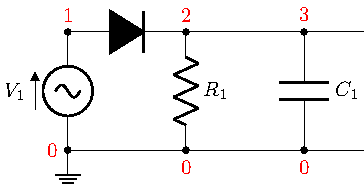
\includegraphics[
  width=0.5\textwidth,
  keepaspectratio
  ]{figuras/figura01.pdf} 
  \captionsetup{width=0.8\textwidth,justification=centering,labelfont=bf,textfont=it,format=plain,labelformat=default,labelsep=period,font=small,name=Figura\,}
  \caption{Valores de amplitude para uma onda sinusoidal ca.}
\end{figure}

\subsection{Rectificadores de Onda Completa}


\begin{itemize}
    \item \newcount\zz
                \loop
                Olá, mundo!!!\cite{horowitz2015art,boylestad2012electronic,floyd2007electronic}
                \advance\zz1
                \ifnum\zz<10
                \repeat
    \item \newcount\zz
                \loop
                Olá, mundo!!!\cite{horowitz2015art,boylestad2012electronic,floyd2007electronic}
                \advance\zz1
                \ifnum\zz<10
                \repeat 
\end{itemize}



%%%%%%%%%%%%%%%%%%%%%%%%%%%%%%%%%%%%%%%%%%%%%%%%%%%%
\lstset{
    language={bash},
    basicstyle=\ttfamily\small,
    breaklines=true,
    breakatwhitespace=false,
    showstringspaces=false,
    columns=flexible
}
\begin{tcolorbox}[
    colback=gray!10,
    colframe=black,
    title={Modelo Spice do Díodo 1N4007},
    breakable
]
\begin{lstlisting}
* SPICE model rectifier diode ***1N4007***
* Use the symbol file ***1n4007.asy***
*
* (c) Diotec Semiconductor AG
* www.diotec.com
* 2017-11-21
*
*********************************************************
* This model is for simulation purposes only. It does *
* not replace reviewing of the data sheet nor real life *
* testing of the part inside the application. *
*********************************************************
*
.subckt 1N4007 A K params: Vrrm=1000 Vrsm=1000 Ir=5u Irsm=5u Vf=1.1 Ifav=1 Rs=.05 trr=1500n Cj=15p Eg=1.11 Xti=3
* Above values are an example for the ***1N4007***. Using the symbol
* above symbol file allows for direct insertion of other values
* according to these data sheet parameters:
*
* Vrrm Repetitive peak reverse voltage
* Ir Leakage current
* Vrsm Surge peak reverse voltage / Reverse avalanche breakdown voltage
* Irsm Defined at avalanche diodes, otherwise set Irsm = Ir
* Vf Forward voltage
* Ifav Test current for Vf, usually equal to average forward rectified current
* trr Reverse recovery time; for Schottky, set trr=5n
* Cj Junction capacitance at 4V
*
* Activation energy: Eg=1.11 for Si (pn) rectifier, Eg=.69 for Schottky (metal barrier) rectifier
* Series resistance: Rs=(Vf@3*Ifav - Vf@Ifav)/(3*Ifav - Ifav) from data sheet curve
* Sat.-current temp. exp: Xti=3 for Si (pn) rectifier, Xti=2 for Schottky (metal barrier) rectifier
D A K Rectifier
.model Rectifier D(Is={Ir/40} Bv={Vrsm*1.05} Ibv={Ir} Vpk=Vrrm N={.8*Vf/25m/(ln(Ifav)-ln(Ir/40))} Rs={Rs} Eg={Eg} Xti={Xti} Iave={Ifav} Cjo={Cj*2} M=.33 Tt={trr} Vp=.5 mfg=Diotec type=Rectifier)
.ends
\end{lstlisting}
\end{tcolorbox}
%%%%%%%%%%%%%%%%%%%%%%%%%%%%%%%%%%%%%%%%%%%%%%%%%%%%


% \printbibliography
\printbibliography[title={Referências}]

\newpage


%%%%%%%%%%%%%%%%%%%%%%%%%%%%%%%%%%%%%%%%%%%%%%%%
%%%%%%%%%%%%%%%%%%%%%%%%%%%%%%%%%%%%%%%%%%%%%%%%

\appendix
\appendixpage

%%%%%%%%%%%%%%%%%%%%%%%%%%%%%%%%%%%%%%%%%%%%%%%%
%%%%%%%%%%%%%%%%%%%%%%%%%%%%%%%%%%%%%%%%%%%%%%%%

\section{Validação de um modelo SPICE do díodo 1N4007}

\newpage

%%%%%%%%%%%%%%%%%%%%%%%%%%%%%%%%%%%%%%%%%%%%%%%%
%%%%%%%%%%%%%%%%%%%%%%%%%%%%%%%%%%%%%%%%%%%%%%%%

\section{Outra coisa qualquer}


%%%%%%%%%%%%%%%%%%%%%%%%%%%%%%%%%%%%%%%%%%%%%%%%
%%%%%%%%%%%%%%%%%%%%%%%%%%%%%%%%%%%%%%%%%%%%%%%%



\label{fim}\end{document}



